\section{Results}
\subsection{Accuracy--sparsity tradeoff}
\label{sec:accuracy}
All 32 C configurations evaluate 82 halos without failures. Independent checks of the saved masks confirm that all 2,296 non-full selections preserve reciprocal membership and architecture loops, retain exactly $\lceil qP\rceil$ pairs, and leave no physical isolates. This is a statement about graph validity and budget accounting, not predictive superiority. At $q=0.4$, mean physical-pair retention is 40.30\%, while mean stored-column retention is 46.69\%. These are means of per-graph fractions; loops and integer rounding explain the distinction.

\begin{table*}[t]
\centering\small
\caption{Test RMSE (dex) on the same 82 halos using the frozen backbone. Column headings denote requested pair retention; the full-graph row always retains 100\%. All non-full rows share the exact decoder and no-isolate constraint. Values are point estimates from one campaign, without seed replication.}
\label{tab:accuracy}
\begin{tabular}{lrrrr}
\toprule
Method & 40\% & 60\% & 80\% & 100\% \\
\midrule
Full graph & 0.114797 & 0.114797 & 0.114797 & 0.114797 \\
Random & 0.156571 & 0.128369 & 0.118196 & 0.114797 \\
Distance & 0.169469 & 0.135384 & 0.117740 & 0.114797 \\
Degree & 0.151941 & 0.132786 & 0.119166 & 0.114797 \\
Stellar binding & 0.208129 & 0.147724 & 0.119173 & 0.114797 \\
Gradient $\times$ input & 0.136900 & 0.137050 & 0.122469 & 0.114797 \\
Trained selector & 0.147382 & 0.133855 & 0.125910 & 0.114797 \\
RL policy & 0.136160 & 0.127760 & 0.121663 & 0.114797 \\
\bottomrule
\end{tabular}

\end{table*}

\begin{figure}[t]
\centering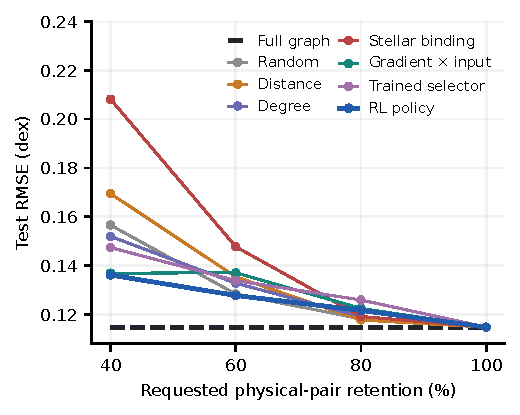
\includegraphics[width=\columnwidth]{figures/accuracy_tradeoff.pdf}
\caption{Accuracy across requested pair budgets (C). The full graph is a reference, not a sparsified mask at each abscissa. Lines join measured configurations; no unmeasured budgets or uncertainty bands are implied.}
\label{fig:tradeoff}
\end{figure}

Table~\ref{tab:accuracy} and Figure~\ref{fig:tradeoff} show convergence toward full-graph performance as retention increases. Full-graph RMSE is $0.114797\dex$. RL at 40\% gives $0.136160\dex$, an 18.61\% increase in error. Its MAE is $0.109011\dex$ and $R^2=0.874075$, compared with $0.090928\dex$ and 0.910491 for the full graph. Removing roughly 60\% of physical pairs therefore has a measurable accuracy cost for this predictor.

The strongest point-estimate sparse selector changes with budget. RL gives $0.127760\dex$ at 60\%, slightly below random's $0.128369\dex$ (a 0.47\% relative difference). At 80\%, distance gives $0.117740\dex$, below RL's $0.121663\dex$. At 100\% every selector recovers the full-graph result within floating-point noise. This is a useful consistency check on decoding and evaluation, but does not demonstrate that a selector generalizes. Gradient saliency is slightly non-monotone between 40\% and 60\%; more retained pairs need not monotonically improve each method's error under a frozen nonlinear predictor.

\subsection{Comparison with alternative selectors}
\label{sec:comparisons}
At 40\%, gradient~$\times$~input is the closest point-estimate competitor: $0.136900\dex$, versus RL's $0.136160\dex$. RL's relative RMSE advantage is approximately 0.54\%, and its MAE is slightly worse ($0.109011$ versus $0.108918\dex$). Thus even the aggregate metric chosen for ranking affects the descriptive conclusion. The trained selector gives $0.147382\dex$ and random gives $0.156571\dex$.

\begin{table*}[t]
\centering\small
\caption{Exploratory paired comparisons at $q=0.4$. $\Delta=\RMSE_{\mathrm{RL}}-\RMSE_{\mathrm{control}}$; negative favors RL. Intervals use 50,000 paired BCa draws. Two-sided permutation tests swap squared errors within halos (99,999 draws). Holm values adjust seven comparisons; intervals remain unadjusted.}
\label{tab:paired}
\begin{tabular}{lrrrr}
\toprule
Control & $\Delta$ (dex) & Marginal 95\% BCa interval (dex) & Paired $p$ & Holm $p$ (7) \\
\midrule
Gradient $\times$ input & -0.000739 & [-0.014508, +0.013582] & 0.91920 & 0.91920 \\
Random & -0.020411 & [-0.050979, +0.003193] & 0.18190 & 0.54570 \\
Trained selector & -0.011222 & [-0.022461, -0.001826] & 0.03774 & 0.15096 \\
Degree & -0.015781 & [-0.043872, +0.006982] & 0.26796 & 0.54570 \\
Distance & -0.033309 & [-0.057936, -0.008931] & 0.01550 & 0.07750 \\
Stellar binding & -0.071968 & [-0.095711, -0.044928] & 0.00004 & 0.00028 \\
Full graph & +0.021364 & [+0.011135, +0.032705] & 0.00022 & 0.00132 \\
\bottomrule
\end{tabular}

\end{table*}

\begin{figure}[t]
\centering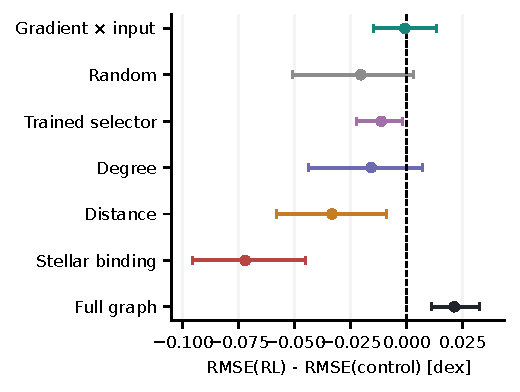
\includegraphics[width=\columnwidth]{figures/paired_uncertainty.pdf}
\caption{Paired RMSE contrasts and marginal 95\% BCa intervals at 40\% retention. Zero denotes equal RMSE. Intervals reflect halo-sample variation conditional on this policy, backbone, catalog, and split.}
\label{fig:paired}
\end{figure}

The paired RL--saliency RMSE difference is $-0.000739\dex$ with 95\% BCa interval $[-0.014508,+0.013582]\dex$ and permutation $p=0.9192$ (Table~\ref{tab:paired}; Figure~\ref{fig:paired}). The interval admits both benefit and harm. RL improves absolute error on 42 of 82 halos and worsens it on 40. A leave-one-halo-out analysis can reverse the sign of the RMSE gap. The observed difference is therefore unsuitable as evidence of a reliable advantage.

Against the single random test realization, the point difference is $-0.020411\dex$ (13.04\% relative improvement), but its interval $[-0.050979,+0.003193]\dex$ crosses zero and $p=0.1819$. Nominal contrasts with the trained selector and distance do not survive the seven-comparison Holm adjustment. The weak stellar-binding heuristic is clearly worse in this conditional analysis; beating it does not establish superiority over competitive selectors. The full graph is more accurate, with RL--full difference $+0.021364\dex$ and interval $[+0.011135,+0.032705]\dex$. Adjusting all 21 sparse-budget contrasts leaves the RL--full and RL--binding conclusions at 40\% below 0.05, while weakening other comparisons. These statements remain conditional on the sampling assumptions in Section~\ref{sec:stats}.

\subsection{Test-time adaptation}
\label{sec:tta}
D preserves exactly the same final pair counts across $K$ for each test halo. Its nominal 50\% budget realizes 51.01\% mean physical retention. The CSV's 56.25\% stored retention includes loops and must not be interpreted as the physical-pair fraction. All 82 test graphs pass the final budget and coverage checks.

\begin{table*}[t]
\centering\small
\caption{D adaptation at a separate requested 50\% pair budget. RMSE is in dex. $K$ is a maximum; early stopping reduces actual steps. $K=20$ was selected using validation only. Nine decimals expose the near-tie between $K=10$ and 20 and are not a claim of measurement precision.}
\label{tab:tta}
\begin{tabular}{rrrrr}
\toprule
$K$ & Validation RMSE & Test RMSE & s/halo & Steps \\
\midrule
0 & 0.127539232 & 0.131123230 & 0.468 & 0.00 \\
5 & 0.127231658 & 0.130803317 & 1.035 & 4.76 \\
10 & 0.127205506 & 0.130391479 & 1.166 & 6.15 \\
20 & 0.127205476 & 0.130391493 & 1.169 & 6.20 \\
\bottomrule
\end{tabular}

\end{table*}

Validation selects $K=20$; $K=10$ and 20 have essentially identical validation and test scores (Table~\ref{tab:tta}). Relative to $K=0$, selected adaptation lowers test RMSE from 0.131123230 to $0.130391493\dex$, an absolute change of $-0.000731736\dex$ and relative change of 0.558\%. MAE changes from 0.102724284 to $0.102651902\dex$, and $R^2$ from 0.883220 to 0.884520. Early stopping yields 6.20 mean steps at $K=20$. The original validation choice is retained despite the negligible difference from $K=10$; test scores do not determine the choice.

D exports aggregates, counts, and adaptation histories but no final per-halo predictions or residuals. Consequently no paired significance assessment of its small accuracy change is supported. Reducing dropout variability is also not guaranteed to reduce prediction error. These observations are descriptive evidence for the implemented adaptation procedure, not evidence of statistically established improvement or cross-domain robustness.

\subsection{Computational efficiency}
\label{sec:efficiency}
At 40\% retention C's RL inference region averages 0.44026 seconds per halo, versus 0.007839 seconds for the full reference: a $56.16\times$ slowdown. Mean scoring, decoder, and pruned-prediction times are approximately 0.01182, 0.41823, and 0.00844 seconds, respectively; the remaining difference is region overhead. CPU feasibility checks dominate the decoder. The measured pruned forward itself is not faster than the full reference in these small-graph runs. RL slowdowns rise to approximately $71\times$, $78\times$, and $83\times$ at 60, 80, and 100\% retention.

\begin{figure*}[t]
\centering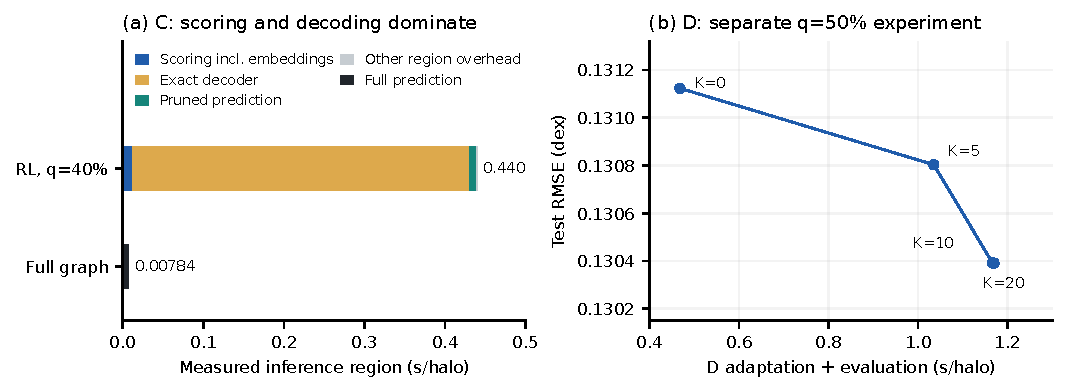
\includegraphics[width=0.96\textwidth]{figures/efficiency_and_tta.pdf}
\caption{Measured computational cost. (a) C's 40\% RL path includes live full-graph embeddings, policy scoring, exact decoding, and retained prediction. (b) D's label-free adaptation at a separate 50\% budget gives a small aggregate RMSE change with higher latency. Timing scopes differ between panels; these are observed campaign measurements, without repeated hardware benchmarking or timing confidence intervals.}
\label{fig:cost}
\end{figure*}

The scorer requires a full-backbone embedding pass before a second, sparse prediction pass. Per-halo records confirm two live predictor forwards for RL versus one for the full reference. Faster decoding alone therefore would not demonstrate an end-to-end speedup over this same backbone. Computation reuse or a cheaper encoder would require a different implemented path and fresh measurements. Graph construction takes 0.8518 seconds for the built split set and is reported separately; recovered historical RL training cost is unknown, not zero.

For D, $K=0$ costs 0.468 seconds per halo and $K=20$ costs 1.169 seconds, a $2.498\times$ latency increase (Figure~\ref{fig:cost}). This cost accompanies a 0.558\% aggregate RMSE reduction without paired uncertainty. No measured amortized speedup, memory reduction, or accuracy--latency deployment advantage is established by these experiments.

\subsection{Additional diagnostics and fine-tuning}
Pair-collapsed physical-alignment analysis gives mean within-halo Spearman correlation 0.376 and median 0.410 between policy keep scores and the stellar binding proxy, with 78/82 positive correlations. This describes association, not causal physical relevance; edges share nodes and the proxy omits most halo matter. No reward or constraint ablation identifies which component causes the predictions.

Thirty-draw dropout intervals constructed as mean $\pm1.96$ standard deviations cover all 82 targets, with mean widths of 1.9596 dex for the full graph and 1.9499 dex for RL. Such broad uncalibrated intervals do not establish useful 95\% calibration or sharp uncertainty. These intervals concern dropout predictions and are distinct from the paired bootstrap intervals above.

B's optional supervised fine-tuning accepts epoch 2 after six executed epochs, because validation pruned RMSE improves from 0.123302 to 0.122764 dex and full-graph validation error remains within the 2\% tolerance. Test accuracy worsens: full RMSE increases from 0.114797 to 0.118644 dex, and pruned RMSE from 0.136160 to 0.137266 dex. One topology-infeasible training graph is excluded from this optional stage (377/378 eligible), without enlarging budgets; the original policy training population remains 378. The negative generalization result is retained, and C's primary comparisons use the unchanged frozen backbone.
